\section{Additional Technical Detail}
\subsection{Retrieval algorithm}
Algorithm~\ref{alg:retrieve} gives the full retrieval of variant B1; B12 and B1QI differ only in the edge weights used by the walk (line 7).

\begin{algorithm}[t]
\caption{Soft-kernel retrieval (variant B1) for one question}
\label{alg:retrieve}
\begin{algorithmic}[1]
\Require question $q$, periods $T_q$, graph $G$, $\lambda{=}1$, $\kappa_{\min}{=}0.05$, $k{=}20$, $B{=}12{,}000$
\State $R_q \gets$ the $3k$ relations most similar to $q$
\ForAll{$f \in R_q$} \Comment{seeding, (\ref{eq:kappa}), (\ref{eq:seed})}
  \State $\kappa_f \gets \max_{t \in T_q} \exp(-\lambda\, d_H(\tau_f, t))$; skip $f$ if $\kappa_f < \kappa_{\min}$
  \State $w(u_f) \gets \max(w(u_f), \kappa_f)$; \; $w(v_f) \gets \max(w(v_f), \kappa_f)$
\EndFor
\If{no seed} \Return $\emptyset$ \EndIf
\State $\bm{\pi} \gets$ PPR with restart $\propto w$, damping 0.85, weights $\omega$ \Comment{(\ref{eq:ppr})}
\State $U \gets$ top-$2k$ entities by $\pi$
\ForAll{edges $(u,v)$, $u, v \in U$, facts $f$ on them with $\kappa(\tau_f) \ge \kappa_{\min}$}
  \State $S(c_f) \gets S(c_f) + \kappa(\tau_f)[\pi(u) + \pi(v)]$ \Comment{(\ref{eq:score})}
\EndFor
\State $S(c) \gets S(c) \cdot \prod_{\gamma \in \Gamma_c}(1 + \gamma)$ for every chunk
\State \Return top-$k$ chunks by $S$, packed greedily within $B$
\end{algorithmic}
\end{algorithm}

\subsection{Kernel weights}
Table~\ref{tab:weights} lists the weights for the locked setting. Facts up to two tree steps away are kept; the boundary case $e^{-3} = 0.0498$ falls just under $\kappa_{\min}$.

\begin{table}[t]
\centering
\caption{Kernel weights for $\lambda = 1$, $\kappa_{\min} = 0.05$}
\label{tab:weights}
\begin{tabular}{lccc}
\toprule
Stored timestamp vs asked period & $d_H$ & $\kappa$ & Used \\
\midrule
inside the asked period & 0 & 1.000 & yes \\
year fact, quarter of the same year asked & 1 & 0.368 & yes \\
neighbouring quarter, same year & 2 & 0.135 & yes \\
year fact, quarter of another year asked & 3 & 0.050 & no \\
neighbouring quarter across a year boundary & 4 & 0.018 & no \\
timestamp not in a valid form & -- & 0 & no \\
\bottomrule
\end{tabular}
\end{table}

\ifextended
\subsection{Noise protocol in detail}
For a fact on entity pair $(u, v)$ with timestamp $\tau$, the first eight bytes of $\operatorname{SHA256}(13 \,\|\, \operatorname{sort}(u, v) \,\|\, \tau)$, read as an integer and divided by $2^{64}$, give $h \in [0, 1)$. If $h < \rho$ the timestamp is moved by one quarter, earlier or later according to the parity of the ninth byte; year-level timestamps move by one year, and month and day timestamps by three months. Because $h$ depends only on the fact, the corrupted graph is identical for every method and every run.

\subsection{Implementation and tests}
The extension consists of four modules: tree distance, kernel and noise (\texttt{soft\_time.py}); the retrieval variants and the run-time swap (\texttt{retriever.py}); model-name mapping for a single provider key (\texttt{openrouter.py}); and a chunk index for naive RAG (\texttt{naive\_index.py}). The scripts answer questions resumably, judge and analyse runs, and rebuild every table and figure from the saved files. The 24 unit tests cover tree paths and distances (5 tests in the soft-time module), the retriever (11 tests, including identity with the base function on a synthetic graph and the $\lambda = 1000$ limit), model mapping (2), the naive index (1), and the hand-check tools (5).

\fi
\section{Additional Results}
\subsection{Development set}
Table~\ref{tab:dev} gives all development runs. The released code scored slightly below our reproduction (0.418 vs 0.445) although the two retrieve the same evidence on 36 of 37 questions; we did not trace the cause of this small difference, and all comparisons use our reproduction, which runs in exactly the same pipeline as the variants. On the three questions where the hard filter found no seed (base-6, base-542, base-519), B1 scored 0.33, 1.00 and 0.40.

\begin{table}[t]
\centering
\caption{Development set (37 questions: 27 answerable, 10 unanswerable), Correct}
\label{tab:dev}
\begin{tabular}{lccc}
\toprule
Run & All & Ans. & Unans. \\
\midrule
TG-RAG, reproduced & 0.445 & 0.425 & 0.500 \\
TG-RAG, released code & 0.418 & 0.388 & 0.500 \\
Naive RAG & 0.488 & 0.336 & 0.900 \\
\textbf{B1, $\lambda = 1$} & \textbf{0.522} & \textbf{0.493} & 0.600 \\
B12 & 0.523 & 0.494 & 0.600 \\
B1QI & 0.506 & 0.434 & 0.700 \\
C & 0.497 & 0.422 & 0.700 \\
BC & 0.511 & 0.404 & 0.800 \\
\midrule
\multicolumn{4}{l}{$\lambda$ sweep (B1, all questions): 0.25: 0.519, 0.5: 0.482,} \\
\multicolumn{4}{l}{1: 0.522, 2: 0.481, 4: 0.456, 1000: 0.447} \\
\bottomrule
\end{tabular}
\end{table}

\subsection{Secondary comparisons and robustness on answerable questions}
Table~\ref{tab:pairs} reports the two pre-registered pairs that do not involve the baseline, and the robustness comparison restricted to answerable questions.

\begin{table}[t]
\centering
\caption{Secondary comparisons (test set)}
\label{tab:pairs}
\resizebox{\linewidth}{!}{%
\begin{tabular}{lcc}
\toprule
Comparison & $\Delta$ all [95\% CI], $p$ & $\Delta$ ans. [95\% CI], $p$ \\
\midrule
B12 vs B1QI & $-0.000$ [$-0.036$, $+0.039$], 0.461 & $+0.008$ [$-0.043$, $+0.058$], 0.368 \\
B12 vs B1 & $+0.001$ [$-0.037$, $+0.044$], 0.435 & $+0.002$ [$-0.045$, $+0.054$], 0.462 \\
B1 vs base, 10\% noise & $-0.018$ [$-0.081$, $+0.043$], 0.719 & $-0.049$ [$-0.123$, $+0.025$], 0.904 \\
B1 vs base, 20\% noise & $+0.031$ [$-0.027$, $+0.096$], 0.155 & $+0.013$ [$-0.059$, $+0.092$], 0.351 \\
B1 vs base, 30\% noise & $+0.061$ [$+0.005$, $+0.120$], 0.019 & $+0.059$ [$-0.004$, $+0.126$], 0.036 \\
\bottomrule
\end{tabular}}
\end{table}

\subsection{Per-question breakdown}
Table~\ref{tab:types} splits the per-question comparison on answerable test questions by type.

\begin{table}[t]
\centering
\caption{B1 vs baseline per answerable test question, by type (exploratory)}
\label{tab:types}
\begin{tabular}{lccccc}
\toprule
Question type & $n$ & Better & Worse & Tied & Net \\
\midrule
Multi-time & 50 & 18 & 7 & 25 & $+4.58$ \\
Single-time, multi-keyword & 30 & 12 & 6 & 12 & $+2.15$ \\
Single-time, multi-company & 22 & 3 & 13 & 6 & $-4.97$ \\
Relative-time & 14 & 2 & 2 & 10 & $-0.13$ \\
\midrule
All answerable & 116 & 35 & 28 & 53 & $+1.63$ \\
\bottomrule
\end{tabular}
\end{table}

\ifextended
\subsection{Reasoning types}
Fig.~\ref{fig:reasoning} splits the test set by what the question asks the model to do. B1 is slightly ahead on comparison questions (0.403 against 0.379, $n = 46$) and on lists of values (0.652 against 0.645, $n = 70$), and identical on questions about periods outside the corpus (0.781, $n = 32$). The largest gap, on unanswerable questions about unreported facts (0.625 against 0.875), rests on only four questions, where one answer moves the score by 0.25; we do not read anything into it.

\begin{figure}[t]
  \centering
  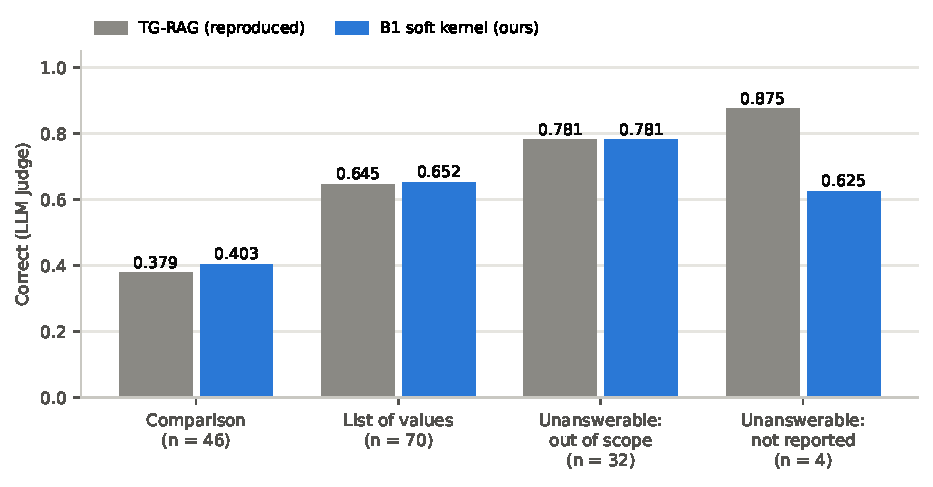
\includegraphics[width=0.85\textwidth]{figures/reasoning_type_test.pdf}
  \caption{Correct by reasoning type, baseline vs B1 (test set, exploratory).}
  \label{fig:reasoning}
\end{figure}

\subsection{Context size and running time}
Fig.~\ref{fig:efficiency} reports the mean number of context tokens sent to the answering model and the mean wall-clock time per question. All graph variants use between 11,039 and 11,462 tokens of the 12,000-token budget, so the variants differ in which facts they send, not in how much text. The timing panel is not a fair speed comparison: the baseline ran first, before the model-call cache was warm (5.94 s per question against 3.13--3.97 s for the later runs), and no separate latency benchmark was made. We therefore make no claim about speed.

\begin{figure}[t]
  \centering
  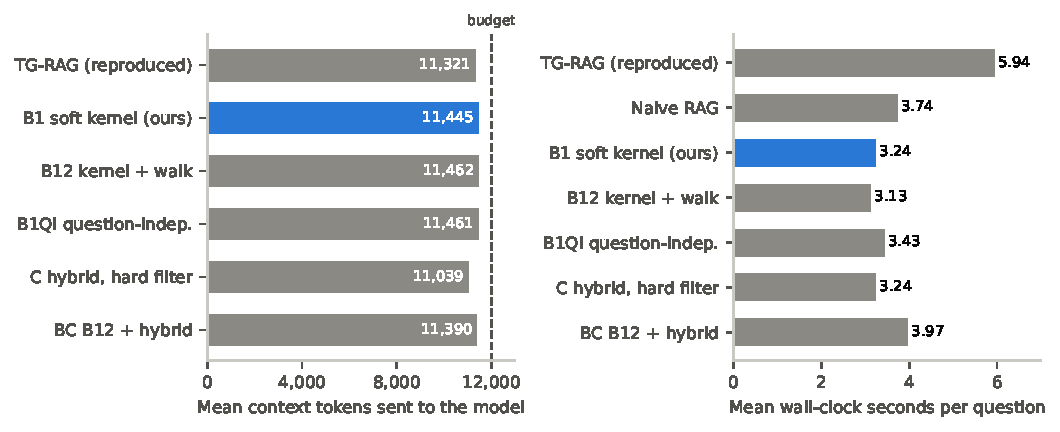
\includegraphics[width=0.95\textwidth]{figures/efficiency_test.pdf}
  \caption{Mean context tokens (left; naive RAG does not record this) and mean wall-clock seconds per question (right) on the test set. Timing differences mainly reflect the response cache, since the baseline ran first.}
  \label{fig:efficiency}
\end{figure}
\fi

\subsection{Case study}
For development question base-6 (EOG Resources' free cash flow in 2021-Q4, 2022-Q1 and 2022-Q2; gold: \$2 billion, \$2.3 billion, nearly \$1.3 billion), the question parser read only 2021-Q4. No candidate carried exactly that quarter, so the baseline kept 0 of 60 candidates and its answer contained three invented figures (judge score 0.00). B1 kept 13 candidates, mostly from 2021-Q1 to Q3 at weight 0.135, sent 11 chunks and answered 2021-Q4 correctly while stating the other quarters were unavailable (0.33). Facts from 2022-Q1 (weight 0.018) and from full years 2020 and 2023 (0.050) were dropped. The missing quarters are a limitation of the shared parser, which we keep unchanged for fairness.

\ifextended
\section{Threats to Validity and Deviations}
\textbf{Internal validity.} The baseline is verified against the released code, every method shares the same graph, parser, prompts and models, and answers are deterministic. The remaining internal threat is the judge: one model with our own prompts. Its agreement with a human reader on 50 blind answers has not yet been measured.

\textbf{External validity.} One benchmark, six companies, one graph and one language-model family; results may differ for other sectors, other graph builders or larger models.

\textbf{Statistical conclusion validity.} The test set gives intervals of about $\pm 0.05$, the robustness result does not survive a multiple-testing correction, and a single noise seed was used.

\textbf{Deviations from the original plan.} The first plan measured robustness on the combined variant BC; the registered comparison uses B1, the variant selected on the development set. A sweep of the B1QI decay rate was planned, but only $\alpha = 1$ was run. A fiscal-year alias for timestamps is implemented but was not enabled. None of these choices was made after seeing test results.

\fi

